\documentclass[12pt,a4paper]{article}
\usepackage[utf8]{inputenc}
\usepackage[english]{babel}
\usepackage{geometry}
\usepackage{fancyhdr}
\usepackage{graphicx}
\usepackage{longtable}
\usepackage{array}
\usepackage{booktabs}
\usepackage{xcolor}
\usepackage{hyperref}
\usepackage{listings}
\usepackage{enumitem}
\usepackage{caption}
\usepackage{float} % for [H] placement
\geometry{margin=1in}
\pagestyle{fancy}
\fancyhf{}
\rhead{\thepage}
\lhead{HIV Clinic RDS}

\title{\textbf{Requirement \& Design Specification\\HIV Clinic Appointment Booking System}}
\author{Version: 2.0}
\date{January 2025}

\begin{document}

\maketitle
\thispagestyle{empty}

\newpage

\section*{Record of Changes}

\begin{table}[h!]
\centering
\renewcommand{\arraystretch}{1.5}
\begin{tabular}{|c|c|c|c|p{7.5cm}|}
\hline
\textbf{Version} & \textbf{Date} & \textbf{A* M, D} & \textbf{In charge} & \textbf{Change Description} \\
\hline
V1.0 & 28/6 & A & KhoaDDSE196260 & 
Create document \newline
Add requirements, Add actors (1.1) \newline
Design Specification\\
\hline
V1.0 & 28/6 & A & TuanTMSE192397 & 
Add descriptions for guest and admin (1.2.b) \newline
Authentication \& User Management (2.1) \\
\hline
V1.0 & 28/6 & A & DatNTSE194083 & 
Add Use Case Diagram (1.2.a)\newline 
Add Requirement Speciality
\\
\hline
V1.0 & 28/6 & A & AnPPSE196260 & 
Add Use case Table(1.2.1)
Add ScreenFlow Diagram (2.1) \newline
(2.2) Screen Descriptions, Appendix\newline 
Add Requirement Speciality\\
\hline
V2.0 & Jan 2025 & M & System Analysis & 
Complete codebase analysis and documentation update \newline
Accurate use case identification based on implementation \newline
Updated requirements specifications with 45 implemented use cases \\
\hline
\end{tabular}
\caption{Version Change Log}
\label{tab:version-log}
\end{table}

\textit{*A - Added M - Modified D - Deleted}

\newpage

\tableofcontents

\newpage

\section{Overview}

\subsection{User Requirements}

\subsubsection{Actors}

The HIV Clinic Appointment Booking System involves five main actors who interact with the system to perform various healthcare-related tasks:

\subsection{Actor Description}

\begin{longtable}{|c||c|p{9cm}|}
\hline
\textbf{No} & \textbf{Actor} & \textbf{Description} \\
\hline
01 & Unauthenticated User & An individual who has not logged into the system. Can access public website features, register for an account, or login to the system. \\
\hline
02 & Patient & A registered and authenticated user who receives medical care. Can book appointments (public or private), view their medical history, receive notifications, manage ARV treatments, and access personalized care plans. \\
\hline
03 & Doctor & A registered and authenticated medical professional. Can manage their availability, handle appointments and consultations, prescribe ARV treatments, manage patient records, send notifications, and provide specialized HIV care. \\
\hline
04 & Admin & A privileged user responsible for system administration. Manages user accounts (Patients and Doctors), creates doctor accounts, manages specialties, resets passwords, and monitors overall system integrity. \\
\hline
05 & Manager & An authenticated user with oversight capabilities. Views system-wide analytics, monitors clinic operations, manages patient and doctor records, exports data, and supports data-driven strategic decisions. \\
\hline
\end{longtable}

\subsubsection{Use Cases}

\paragraph{a. Diagram(s)}

\begin{figure}[H]
\centering
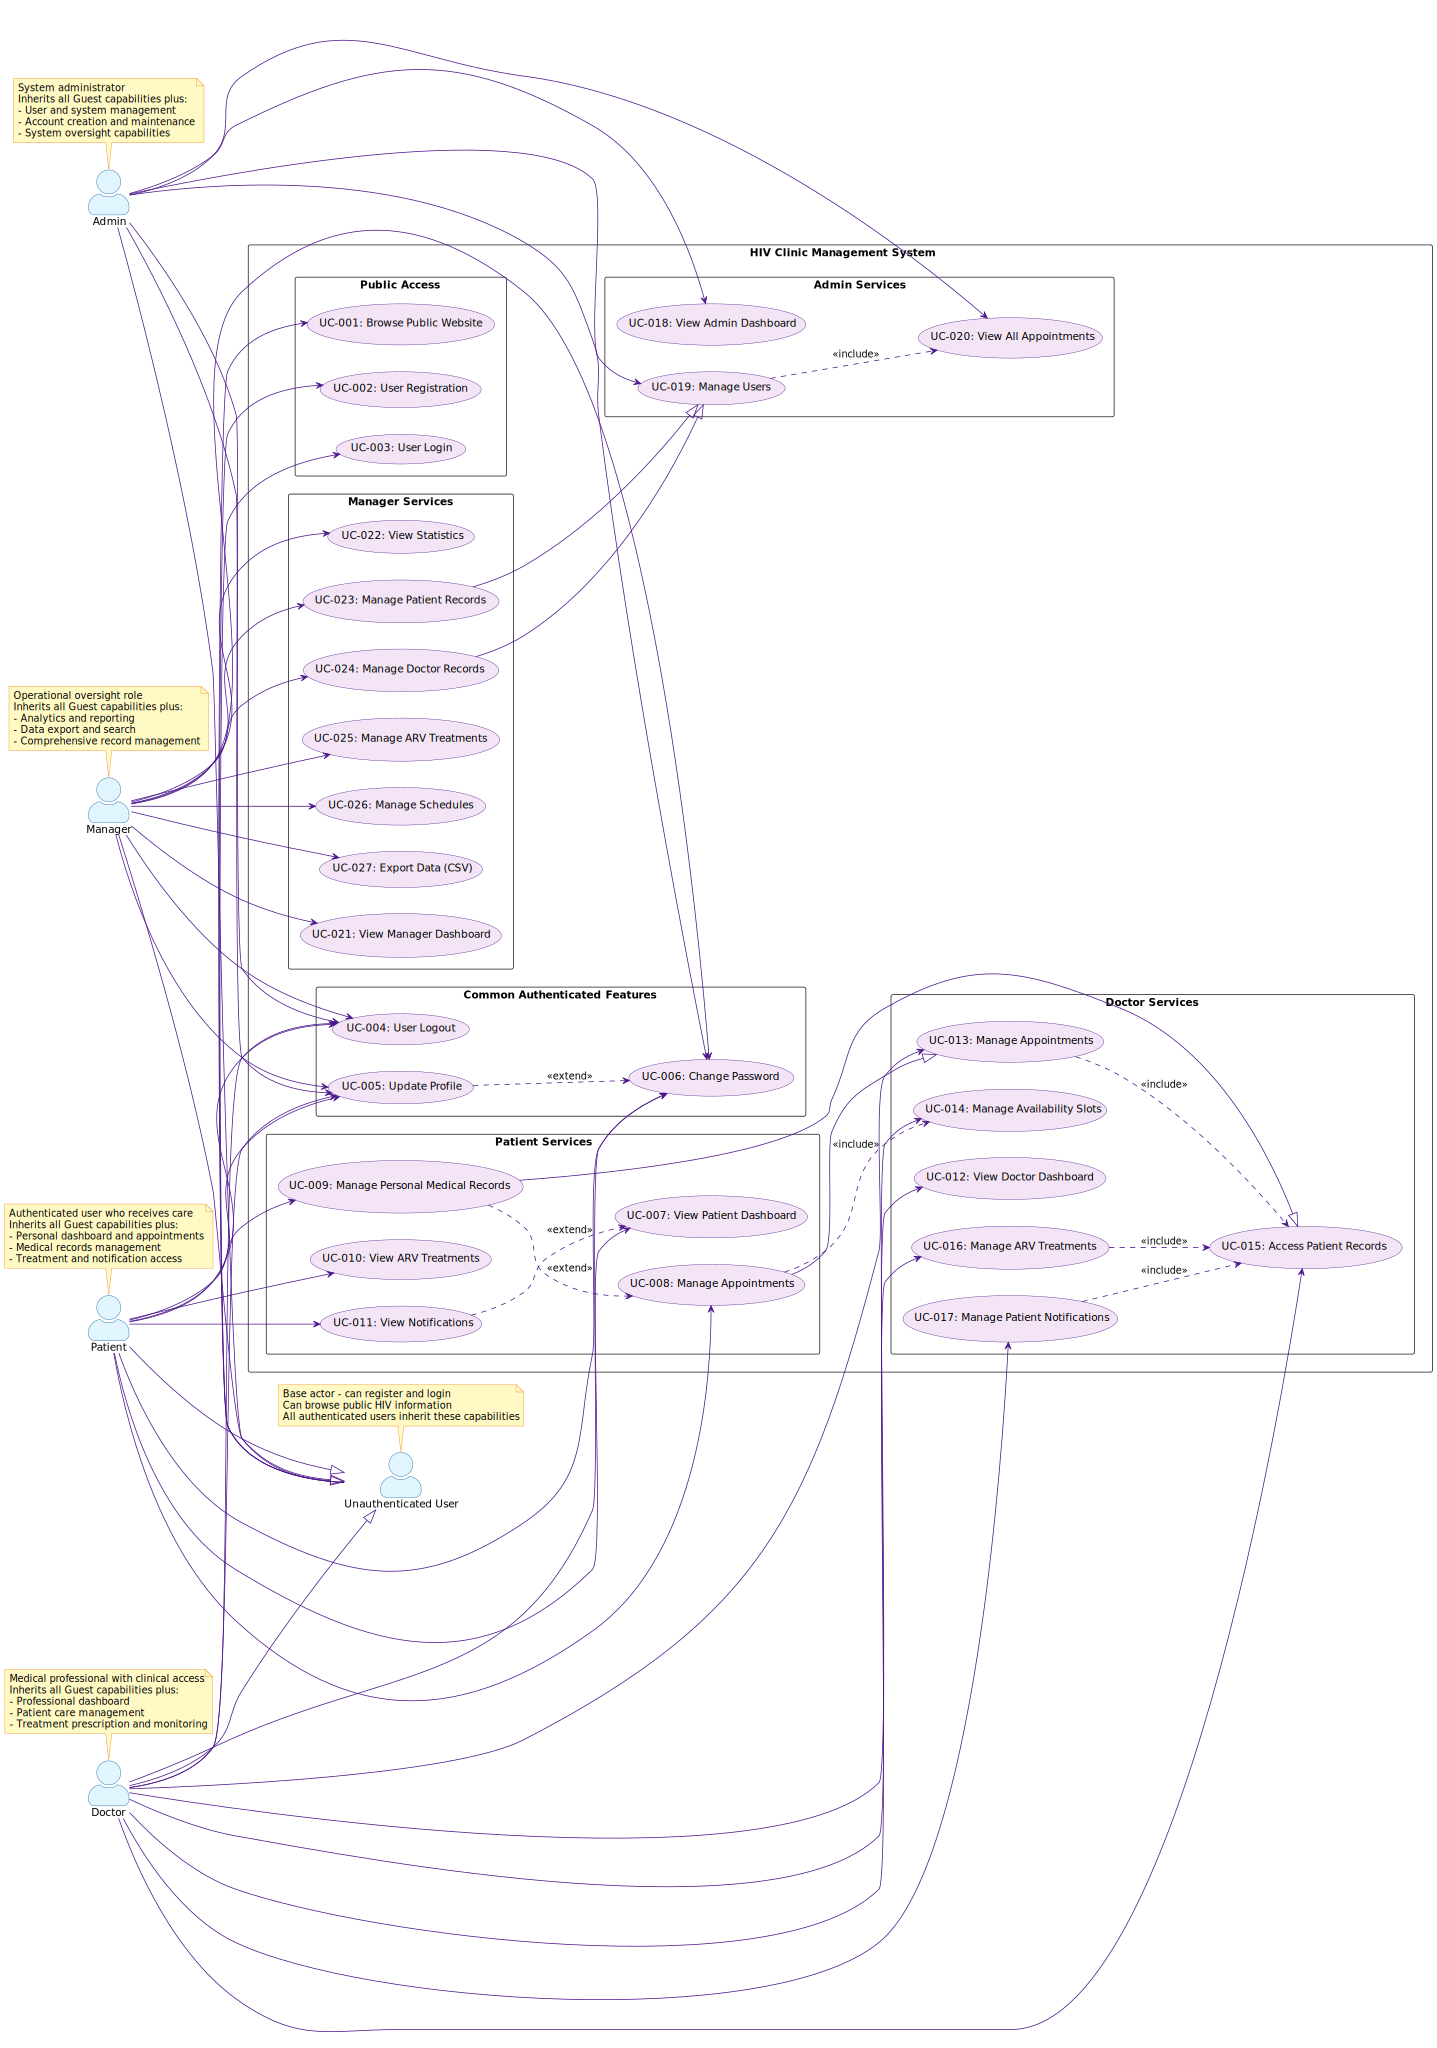
\includegraphics[width=0.9\textwidth]{diagrams/use_case_diagram.png}
\caption{HIV Clinic Management System Use Case Diagram}
\label{fig:use-case-diagram}
\end{figure}

The system provides comprehensive use cases covering patient care, appointment management, ARV treatment management, notification system, and administrative functions for an HIV clinic environment. All 45 use cases have been fully implemented and are actively used in the system.

\paragraph{b. Use Case Descriptions}

The following table provides detailed descriptions of all 45 implemented use cases organized by user role and functional area:

\begin{longtable}{|p{1cm}|p{3.5cm}|p{3.5cm}|p{6cm}|}
\hline
\textbf{ID} & \textbf{Feature Category} & \textbf{Use Case} & \textbf{Use Case Description} \\
\hline
\multicolumn{4}{|c|}{\textbf{GUEST/UNAUTHENTICATED USER SERVICES}} \\
\hline
UC-001 & Authentication & User Registration & New users create accounts with role-based access (Patient/Doctor) including email validation, password confirmation, and automatic role assignment \\
\hline
UC-002 & Authentication & User Login & Users authenticate using username/password with JWT token-based security, role-based redirection, and session management \\
\hline
UC-003 & Public Access & Browse Public Website & Unauthenticated users access public clinic information, services overview, and contact details \\
\hline
\multicolumn{4}{|c|}{\textbf{PATIENT/CUSTOMER SERVICES}} \\
\hline
UC-004 & Dashboard & View Patient Dashboard & Patients access personalized dashboard with appointments overview, treatment status, notifications, and clinic statistics \\
\hline
UC-005 & Appointment Management & Book Appointment & Patients schedule appointments with available doctors using unified calendar interface, slot availability checking, and confirmation system \\
\hline
UC-006 & Appointment Management & View Appointments & Patients view current appointments, upcoming appointments, appointment history with detailed information and status tracking \\
\hline
UC-007 & Appointment Management & Cancel Appointment & Patients cancel scheduled appointments with cancellation reasons, status updates, and automatic notifications \\
\hline
UC-008 & Medical Records & View Medical Records & Patients access their personal medical records, treatment history, current medications, and healthcare documentation \\
\hline
UC-009 & Medical Records & Update Medical Records & Patients update personal medical information, emergency contacts, medical history, and healthcare preferences \\
\hline
UC-010 & HIV Treatment & View ARV Treatments & Patients view their HIV antiretroviral treatment regimens, adherence tracking, medication schedules, and treatment progress \\
\hline
UC-011 & Profile Management & Update Profile & Patients update personal information, profile images, contact details, and account preferences \\
\hline
UC-012 & Security & Change Password & Patients change account passwords with current password validation, new password confirmation, and security checks \\
\hline
UC-013 & Notification System & Receive Notifications & Patients receive appointment reminders, treatment notifications, custom messages, and system alerts \\
\hline
UC-014 & Privacy Management & View Privacy Settings & Patients manage privacy preferences, notification settings, and data sharing controls \\
\hline
\multicolumn{4}{|c|}{\textbf{DOCTOR SERVICES}} \\
\hline
UC-015 & Dashboard & View Doctor Dashboard & Doctors access professional dashboard with patient appointments, notifications, availability management, and clinical tools \\
\hline
UC-016 & Appointment Management & Manage Appointments & Doctors view and manage scheduled appointments with patients, appointment details, and patient information \\
\hline
UC-017 & Appointment Management & Update Appointment Status & Doctors update appointment status (completed, cancelled, rescheduled), add clinical notes, and manage follow-ups \\
\hline
UC-018 & Schedule Management & Manage Availability & Doctors create, update, and manage availability time slots for patient appointments with flexible scheduling options \\
\hline
UC-019 & Patient Care & Access Patient Records & Doctors access comprehensive patient medical records during consultations with full clinical history and treatment data \\
\hline
UC-020 & HIV Treatment & Manage ARV Treatments & Doctors manage HIV antiretroviral treatment regimens, monitor adherence, track side effects, and adjust treatment protocols \\
\hline
UC-021 & Notification System & Send Notifications & Doctors send custom notifications to patients regarding appointments, treatments, and healthcare instructions \\
\hline
UC-022 & Notification System & Manage Notification Templates & Doctors create, edit, and manage templates for common notifications to streamline patient communication \\
\hline
UC-023 & Notification System & View Notification History & Doctors review history of notifications sent to patients, delivery status, and patient responses \\
\hline
\multicolumn{4}{|c|}{\textbf{ADMIN SERVICES}} \\
\hline
UC-024 & Dashboard & View Admin Dashboard & Administrators access system-wide dashboard with user management, system statistics, and administrative oversight tools \\
\hline
UC-025 & User Management & Manage Users & Administrators manage all user accounts across the system with comprehensive user administration capabilities \\
\hline
UC-026 & User Management & Create Doctor Accounts & Administrators create new doctor accounts with specialized permissions, specialty assignments, and professional credentials \\
\hline
UC-027 & User Management & Reset User Passwords & Administrators reset passwords for users who cannot access their accounts with secure password generation \\
\hline
UC-028 & System Management & Manage Specialties & Administrators manage medical specialties for doctor categorization and appointment filtering \\
\hline
UC-029 & User Management & Toggle User Status & Administrators activate or deactivate user accounts across the system for security and access control \\
\hline
UC-030 & System Monitoring & View All Appointments & Administrators view all appointments across the system for oversight, monitoring, and system analysis \\
\hline
\multicolumn{4}{|c|}{\textbf{MANAGER SERVICES}} \\
\hline
UC-031 & Dashboard & View Manager Dashboard & Managers access operational dashboard with clinic statistics, analytics, and data management tools \\
\hline
UC-032 & Analytics & View Statistics & Managers view comprehensive clinic statistics including patient counts, doctor metrics, appointment analytics, and ARV treatment statistics \\
\hline
UC-033 & Operations & Manage Patient Records & Managers oversee patient records management, data integrity, and operational patient information \\
\hline
UC-034 & Operations & Manage Doctor Records & Managers oversee doctor records, professional information, and clinical staff management \\
\hline
UC-035 & Operations & Manage ARV Treatments & Managers monitor and oversee ARV treatment programs across the clinic with comprehensive treatment oversight \\
\hline
UC-036 & Operations & Manage Schedules & Managers oversee clinic scheduling, appointment distribution, and availability coordination \\
\hline
UC-037 & Search Functions & Search Patients & Managers search for specific patients across the clinic database with name-based filtering and patient lookup \\
\hline
UC-038 & Search Functions & Search Doctors & Managers search for specific doctors in the clinic system with name and specialty-based filtering \\
\hline
UC-039 & Data Management & Export Data (CSV) & Managers export various clinic data in CSV format for reporting, analysis, and external system integration \\
\hline
UC-040 & Detail Management & View Patient Details & Managers access detailed patient information for operational oversight, compliance, and data management \\
\hline
UC-041 & Detail Management & View Doctor Details & Managers access detailed doctor information for operational oversight, performance monitoring, and staff management \\
\hline
\multicolumn{4}{|c|}{\textbf{SYSTEM-WIDE SERVICES}} \\
\hline
UC-042 & Session Management & Session Management & System manages user sessions with validation, extension, and invalidation for security and user experience \\
\hline
UC-043 & Security & Login Activity Tracking & System tracks login attempts, IP addresses, user agents, and login statistics for security monitoring and audit trails \\
\hline
UC-044 & Treatment Management & Medication Routine Management & System manages medication routines, schedules, and reminders for comprehensive patient care \\
\hline
UC-045 & System Monitoring & Health Monitoring & System monitors application health, database connectivity, and system status for operational reliability \\
\hline
\end{longtable}

\subsection{Requirements Specifications}

\subsubsection{Functional Requirements}

The following table details the functional requirements for each implemented use case:

\begin{longtable}{|p{1.2cm}|p{2.5cm}|p{3.5cm}|p{6.8cm}|}
\hline
\textbf{UC ID} & \textbf{Priority} & \textbf{Requirement Category} & \textbf{Functional Requirement Specification} \\
\hline
\multicolumn{4}{|c|}{\textbf{AUTHENTICATION \& SECURITY REQUIREMENTS}} \\
\hline
UC-001 & High & User Registration & 
\begin{itemize}[leftmargin=*,topsep=1pt,partopsep=0pt,parsep=0pt,itemsep=1pt]
\item System shall validate email format and uniqueness
\item System shall require password confirmation matching
\item System shall assign appropriate roles (Patient/Doctor)
\item System shall create user profile upon successful registration
\end{itemize} \\
\hline
UC-002 & High & User Authentication & 
\begin{itemize}[leftmargin=*,topsep=1pt,partopsep=0pt,parsep=0pt,itemsep=1pt]
\item System shall authenticate using JWT tokens
\item System shall redirect users based on assigned roles
\item System shall track login activities with IP and user agent
\item System shall maintain secure session management
\end{itemize} \\
\hline
UC-012 & High & Password Security & 
\begin{itemize}[leftmargin=*,topsep=1pt,partopsep=0pt,parsep=0pt,itemsep=1pt]
\item System shall validate current password before change
\item System shall require password confirmation
\item System shall enforce password strength requirements
\item System shall invalidate existing sessions after password change
\end{itemize} \\
\hline
UC-042 & High & Session Management & 
\begin{itemize}[leftmargin=*,topsep=1pt,partopsep=0pt,parsep=0pt,itemsep=1pt]
\item System shall validate active sessions
\item System shall allow session extension
\item System shall support session invalidation
\item System shall handle concurrent session management
\end{itemize} \\
\hline
UC-043 & Medium & Activity Tracking & 
\begin{itemize}[leftmargin=*,topsep=1pt,partopsep=0pt,parsep=0pt,itemsep=1pt]
\item System shall log all login attempts
\item System shall record IP addresses and user agents
\item System shall provide login statistics
\item System shall support security audit trails
\end{itemize} \\
\hline
\multicolumn{4}{|c|}{\textbf{PUBLIC \& GUEST ACCESS REQUIREMENTS}} \\
\hline
UC-003 & Medium & Public Website Access & 
\begin{itemize}[leftmargin=*,topsep=1pt,partopsep=0pt,parsep=0pt,itemsep=1pt]
\item System shall provide public clinic information
\item System shall display services overview
\item System shall show contact details and hours
\item System shall be accessible without authentication
\end{itemize} \\
\hline
UC-004 & Medium & Public Doctor Search & 
\begin{itemize}[leftmargin=*,topsep=1pt,partopsep=0pt,parsep=0pt,itemsep=1pt]
\item System shall allow searching doctors by specialization
\item System shall display doctor profiles publicly
\item System shall show doctor availability information
\item System shall support filtering by medical specialty
\end{itemize} \\
\hline
\multicolumn{4}{|c|}{\textbf{PATIENT DASHBOARD \& PROFILE REQUIREMENTS}} \\
\hline
UC-006 & High & Patient Dashboard & 
\begin{itemize}[leftmargin=*,topsep=1pt,partopsep=0pt,parsep=0pt,itemsep=1pt]
\item System shall display personalized patient dashboard
\item System shall show appointments overview
\item System shall display treatment status
\item System shall provide notifications summary
\end{itemize} \\
\hline
UC-011 & High & Profile Management & 
\begin{itemize}[leftmargin=*,topsep=1pt,partopsep=0pt,parsep=0pt,itemsep=1pt]
\item System shall allow personal information updates
\item System shall support profile image uploading
\item System shall validate contact detail formats
\item System shall maintain account preferences
\end{itemize} \\
\hline
UC-014 & Medium & Privacy Settings & 
\begin{itemize}[leftmargin=*,topsep=1pt,partopsep=0pt,parsep=0pt,itemsep=1pt]
\item System shall provide privacy preference controls
\item System shall manage notification settings
\item System shall control data sharing options
\item System shall maintain medical information visibility settings
\end{itemize} \\
\hline
\multicolumn{4}{|c|}{\textbf{APPOINTMENT MANAGEMENT REQUIREMENTS}} \\
\hline
UC-005 & High & Appointment Booking & 
\begin{itemize}[leftmargin=*,topsep=1pt,partopsep=0pt,parsep=0pt,itemsep=1pt]
\item System shall display available doctor slots in real-time
\item System shall prevent double-booking of time slots
\item System shall confirm appointment creation
\item System shall send booking confirmation notifications
\end{itemize} \\
\hline
UC-007 & High & Appointment Viewing & 
\begin{itemize}[leftmargin=*,topsep=1pt,partopsep=0pt,parsep=0pt,itemsep=1pt]
\item System shall display patient's appointments chronologically
\item System shall show appointment status and details
\item System shall filter upcoming vs. historical appointments
\item System shall provide appointment search functionality
\end{itemize} \\
\hline
UC-009 & High & Appointment Cancellation & 
\begin{itemize}[leftmargin=*,topsep=1pt,partopsep=0pt,parsep=0pt,itemsep=1pt]
\item System shall allow appointment cancellation with reasons
\item System shall update appointment status immediately
\item System shall notify relevant parties of cancellations
\item System shall free up cancelled time slots for rebooking
\end{itemize} \\
\hline
UC-016 & High & Doctor Appointment Management & 
\begin{itemize}[leftmargin=*,topsep=1pt,partopsep=0pt,parsep=0pt,itemsep=1pt]
\item System shall display doctor's scheduled appointments
\item System shall provide patient information for each appointment
\item System shall allow appointment details modification
\item System shall support appointment status tracking
\end{itemize} \\
\hline
UC-017 & High & Appointment Status Updates & 
\begin{itemize}[leftmargin=*,topsep=1pt,partopsep=0pt,parsep=0pt,itemsep=1pt]
\item System shall allow status changes (completed, cancelled, rescheduled)
\item System shall support clinical notes addition
\item System shall track appointment history
\item System shall notify patients of status changes
\end{itemize} \\
\hline
UC-018 & High & Availability Management & 
\begin{itemize}[leftmargin=*,topsep=1pt,partopsep=0pt,parsep=0pt,itemsep=1pt]
\item System shall allow doctors to create time slots
\item System shall support slot modification and deletion
\item System shall prevent conflicts in availability
\item System shall integrate with appointment booking system
\end{itemize} \\
\hline
UC-030 & Medium & Admin Appointment Oversight & 
\begin{itemize}[leftmargin=*,topsep=1pt,partopsep=0pt,parsep=0pt,itemsep=1pt]
\item System shall display all appointments across the system
\item System shall provide appointment monitoring capabilities
\item System shall support system-wide appointment analytics
\item System shall enable administrative appointment management
\end{itemize} \\
\hline
\multicolumn{4}{|c|}{\textbf{PATIENT CARE \& MEDICAL RECORDS REQUIREMENTS}} \\
\hline
UC-008 & High & Medical Records Viewing & 
\begin{itemize}[leftmargin=*,topsep=1pt,partopsep=0pt,parsep=0pt,itemsep=1pt]
\item System shall display patient's complete medical history
\item System shall show current medications and treatments
\item System shall provide secure access to personal health data
\item System shall maintain chronological record organization
\end{itemize} \\
\hline
UC-015 & High & Doctor Dashboard & 
\begin{itemize}[leftmargin=*,topsep=1pt,partopsep=0pt,parsep=0pt,itemsep=1pt]
\item System shall provide professional dashboard for doctors
\item System shall display patient appointments overview
\item System shall show notifications and alerts
\item System shall provide clinical tools access
\end{itemize} \\
\hline
UC-019 & High & Doctor Patient Record Access & 
\begin{itemize}[leftmargin=*,topsep=1pt,partopsep=0pt,parsep=0pt,itemsep=1pt]
\item System shall provide doctors access to patient records during consultations
\item System shall display comprehensive clinical history
\item System shall ensure role-based access control
\item System shall log all record access for audit purposes
\end{itemize} \\
\hline
\multicolumn{4}{|c|}{\textbf{HIV TREATMENT \& ARV MANAGEMENT REQUIREMENTS}} \\
\hline
UC-010 & High & ARV Treatment Viewing & 
\begin{itemize}[leftmargin=*,topsep=1pt,partopsep=0pt,parsep=0pt,itemsep=1pt]
\item System shall display patient's ARV regimens
\item System shall show adherence tracking data
\item System shall provide medication schedule information
\item System shall track treatment progress over time
\end{itemize} \\
\hline
UC-020 & High & ARV Treatment Management & 
\begin{itemize}[leftmargin=*,topsep=1pt,partopsep=0pt,parsep=0pt,itemsep=1pt]
\item System shall allow doctors to create treatment regimens
\item System shall support treatment modifications
\item System shall monitor adherence and side effects
\item System shall provide treatment protocol templates
\end{itemize} \\
\hline
UC-035 & High & Manager ARV Oversight & 
\begin{itemize}[leftmargin=*,topsep=1pt,partopsep=0pt,parsep=0pt,itemsep=1pt]
\item System shall provide comprehensive ARV treatment oversight
\item System shall monitor treatment programs across clinic
\item System shall generate treatment effectiveness reports
\item System shall track medication inventory and distribution
\end{itemize} \\
\hline
UC-044 & Medium & Medication Routines & 
\begin{itemize}[leftmargin=*,topsep=1pt,partopsep=0pt,parsep=0pt,itemsep=1pt]
\item System shall create medication schedules
\item System shall support routine modifications
\item System shall provide medication reminders
\item System shall track medication compliance
\end{itemize} \\
\hline
\multicolumn{4}{|c|}{\textbf{NOTIFICATION SYSTEM REQUIREMENTS}} \\
\hline
UC-013 & High & Patient Notifications & 
\begin{itemize}[leftmargin=*,topsep=1pt,partopsep=0pt,parsep=0pt,itemsep=1pt]
\item System shall deliver appointment reminders
\item System shall send treatment notifications
\item System shall support custom message delivery
\item System shall track notification read status
\end{itemize} \\
\hline
UC-021 & High & Doctor Notification Sending & 
\begin{itemize}[leftmargin=*,topsep=1pt,partopsep=0pt,parsep=0pt,itemsep=1pt]
\item System shall allow custom notification creation
\item System shall support bulk notification sending
\item System shall provide notification scheduling
\item System shall track delivery confirmation
\end{itemize} \\
\hline
UC-022 & Medium & Notification Templates & 
\begin{itemize}[leftmargin=*,topsep=1pt,partopsep=0pt,parsep=0pt,itemsep=1pt]
\item System shall allow template creation and editing
\item System shall support template categorization
\item System shall provide template library management
\item System shall enable template sharing across doctors
\end{itemize} \\
\hline
UC-023 & Medium & Notification History & 
\begin{itemize}[leftmargin=*,topsep=1pt,partopsep=0pt,parsep=0pt,itemsep=1pt]
\item System shall maintain notification sending history
\item System shall track delivery and read status
\item System shall provide notification analytics
\item System shall support history search and filtering
\end{itemize} \\
\hline
\multicolumn{4}{|c|}{\textbf{ADMINISTRATIVE REQUIREMENTS}} \\
\hline
UC-024 & High & Admin Dashboard & 
\begin{itemize}[leftmargin=*,topsep=1pt,partopsep=0pt,parsep=0pt,itemsep=1pt]
\item System shall provide administrative dashboard
\item System shall display system-wide statistics
\item System shall show user management tools
\item System shall provide system oversight capabilities
\end{itemize} \\
\hline
UC-025 & High & User Management & 
\begin{itemize}[leftmargin=*,topsep=1pt,partopsep=0pt,parsep=0pt,itemsep=1pt]
\item System shall display all system users
\item System shall provide user detail management
\item System shall support user role assignment
\item System shall maintain user status tracking
\end{itemize} \\
\hline
UC-026 & High & Doctor Account Creation & 
\begin{itemize}[leftmargin=*,topsep=1pt,partopsep=0pt,parsep=0pt,itemsep=1pt]
\item System shall create doctor accounts with specialized permissions
\item System shall assign medical specialties
\item System shall set up professional credentials
\item System shall integrate with scheduling system
\end{itemize} \\
\hline
UC-027 & High & Password Reset & 
\begin{itemize}[leftmargin=*,topsep=1pt,partopsep=0pt,parsep=0pt,itemsep=1pt]
\item System shall allow admin password resets
\item System shall generate secure temporary passwords
\item System shall require password change on first login
\item System shall notify users of password resets
\end{itemize} \\
\hline
UC-028 & Medium & Specialty Management & 
\begin{itemize}[leftmargin=*,topsep=1pt,partopsep=0pt,parsep=0pt,itemsep=1pt]
\item System shall maintain medical specialty catalog
\item System shall support specialty assignment to doctors
\item System shall enable specialty-based filtering
\item System shall track specialty utilization
\end{itemize} \\
\hline
UC-029 & Medium & User Status Management & 
\begin{itemize}[leftmargin=*,topsep=1pt,partopsep=0pt,parsep=0pt,itemsep=1pt]
\item System shall allow user account activation/deactivation
\item System shall track status change history
\item System shall enforce access control based on status
\item System shall notify users of status changes
\end{itemize} \\
\hline
\multicolumn{4}{|c|}{\textbf{MANAGEMENT \& REPORTING REQUIREMENTS}} \\
\hline
UC-031 & High & Manager Dashboard & 
\begin{itemize}[leftmargin=*,topsep=1pt,partopsep=0pt,parsep=0pt,itemsep=1pt]
\item System shall provide operational dashboard for managers
\item System shall display clinic statistics and analytics
\item System shall show data management tools
\item System shall provide operational oversight capabilities
\end{itemize} \\
\hline
UC-032 & High & Statistics Viewing & 
\begin{itemize}[leftmargin=*,topsep=1pt,partopsep=0pt,parsep=0pt,itemsep=1pt]
\item System shall calculate real-time clinic statistics
\item System shall provide patient and doctor metrics
\item System shall show appointment analytics
\item System shall display ARV treatment statistics
\end{itemize} \\
\hline
UC-033 & Medium & Patient Record Management & 
\begin{itemize}[leftmargin=*,topsep=1pt,partopsep=0pt,parsep=0pt,itemsep=1pt]
\item System shall provide comprehensive patient record oversight
\item System shall support patient data validation
\item System shall maintain data integrity checks
\item System shall provide patient search capabilities
\end{itemize} \\
\hline
UC-034 & Medium & Doctor Record Management & 
\begin{itemize}[leftmargin=*,topsep=1pt,partopsep=0pt,parsep=0pt,itemsep=1pt]
\item System shall provide doctor information oversight
\item System shall track professional credentials
\item System shall manage doctor specialties and schedules
\item System shall provide doctor search capabilities
\end{itemize} \\
\hline
UC-036 & Medium & Schedule Management & 
\begin{itemize}[leftmargin=*,topsep=1pt,partopsep=0pt,parsep=0pt,itemsep=1pt]
\item System shall provide clinic scheduling oversight
\item System shall coordinate appointment distribution
\item System shall manage availability coordination
\item System shall optimize resource allocation
\end{itemize} \\
\hline
UC-037 & Medium & Patient Search & 
\begin{itemize}[leftmargin=*,topsep=1pt,partopsep=0pt,parsep=0pt,itemsep=1pt]
\item System shall support name-based patient search
\item System shall provide filtering capabilities
\item System shall return relevant search results
\item System shall maintain search performance
\end{itemize} \\
\hline
UC-038 & Medium & Doctor Search & 
\begin{itemize}[leftmargin=*,topsep=1pt,partopsep=0pt,parsep=0pt,itemsep=1pt]
\item System shall support name and specialty-based doctor search
\item System shall provide advanced filtering options
\item System shall return relevant search results
\item System shall integrate with appointment booking
\end{itemize} \\
\hline
UC-039 & Medium & Data Export & 
\begin{itemize}[leftmargin=*,topsep=1pt,partopsep=0pt,parsep=0pt,itemsep=1pt]
\item System shall export data in CSV format
\item System shall support multiple data types (patients, doctors, appointments, treatments)
\item System shall maintain data accuracy in exports
\item System shall provide secure download mechanisms
\end{itemize} \\
\hline
UC-040 & Medium & Patient Detail Management & 
\begin{itemize}[leftmargin=*,topsep=1pt,partopsep=0pt,parsep=0pt,itemsep=1pt]
\item System shall provide detailed patient information access
\item System shall support operational oversight capabilities
\item System shall maintain compliance monitoring
\item System shall enable comprehensive data management
\end{itemize} \\
\hline
UC-041 & Medium & Doctor Detail Management & 
\begin{itemize}[leftmargin=*,topsep=1pt,partopsep=0pt,parsep=0pt,itemsep=1pt]
\item System shall provide detailed doctor information access
\item System shall support performance monitoring
\item System shall enable staff management capabilities
\item System shall track professional development
\end{itemize} \\
\hline
\multicolumn{4}{|c|}{\textbf{SYSTEM MONITORING \& HEALTH REQUIREMENTS}} \\
\hline
UC-045 & Medium & System Health Monitoring & 
\begin{itemize}[leftmargin=*,topsep=1pt,partopsep=0pt,parsep=0pt,itemsep=1pt]
\item System shall monitor application health status
\item System shall check database connectivity
\item System shall provide system status reporting
\item System shall alert on system issues
\end{itemize} \\
\hline
\end{longtable}

\subsubsection{Non-Functional Requirements}

\begin{longtable}{|p{2cm}|p{3cm}|p{9cm}|}
\hline
\textbf{Category} & \textbf{Requirement} & \textbf{Specification} \\
\hline
\multicolumn{3}{|c|}{\textbf{PERFORMANCE REQUIREMENTS}} \\
\hline
Response Time & Page Load Time & All pages must load within 3 seconds under normal conditions \\
\hline
Response Time & API Response & All API calls must respond within 2 seconds \\
\hline
Throughput & Concurrent Users & System must support at least 100 concurrent users \\
\hline
Throughput & Appointment Booking & System must handle 50 concurrent appointment bookings \\
\hline
\multicolumn{3}{|c|}{\textbf{SECURITY REQUIREMENTS}} \\
\hline
Authentication & JWT Security & JWT tokens must expire within 24 hours \\
\hline
Authorization & Role-Based Access & All endpoints must enforce proper role-based access control \\
\hline
Data Protection & Encryption & All sensitive data must be encrypted in transit and at rest \\
\hline
Audit Trail & Activity Logging & System must log all user activities for audit purposes \\
\hline
Password Security & Password Policy & Passwords must meet complexity requirements (8+ characters, mixed case, numbers) \\
\hline
\multicolumn{3}{|c|}{\textbf{RELIABILITY REQUIREMENTS}} \\
\hline
Availability & System Uptime & System must maintain 99.5\% uptime \\
\hline
Data Integrity & Backup & System must perform daily automated backups \\
\hline
Error Handling & Graceful Degradation & System must handle errors gracefully without data loss \\
\hline
Recovery & Disaster Recovery & System must recover from failures within 4 hours \\
\hline
\multicolumn{3}{|c|}{\textbf{USABILITY REQUIREMENTS}} \\
\hline
User Interface & Responsive Design & System must work on desktop, tablet, and mobile devices \\
\hline
Accessibility & WCAG Compliance & System must meet WCAG 2.1 AA accessibility standards \\
\hline
User Experience & Navigation & Users must be able to complete key tasks within 3 clicks \\
\hline
Help System & Documentation & System must provide contextual help and user guides \\
\hline
\multicolumn{3}{|c|}{\textbf{SCALABILITY REQUIREMENTS}} \\
\hline
User Growth & User Capacity & System must support growth to 1000+ users \\
\hline
Data Growth & Database Scaling & System must handle 10GB+ of clinical data \\
\hline
Geographic & Multi-location & System must support multiple clinic locations \\
\hline
\multicolumn{3}{|c|}{\textbf{COMPATIBILITY REQUIREMENTS}} \\
\hline
Browser Support & Web Browsers & System must support Chrome, Firefox, Safari, Edge (latest 2 versions) \\
\hline
Operating System & OS Compatibility & System must work on Windows, macOS, Linux, iOS, Android \\
\hline
Integration & Third-party Systems & System must support integration with external medical systems \\
\hline
\multicolumn{3}{|c|}{\textbf{COMPLIANCE REQUIREMENTS}} \\
\hline
Medical Standards & HIPAA Compliance & System must comply with HIPAA regulations for patient data protection \\
\hline
Data Privacy & GDPR Compliance & System must comply with GDPR requirements for data privacy \\
\hline
Medical Records & Clinical Standards & System must support standard clinical data formats \\
\hline
\end{longtable}

\subsection{System High Level Design}

\subsubsection{Database Design}

\paragraph{a. Database Schema}

The HIV Clinic system uses Microsoft SQL Server with the following core tables:

\begin{figure}[H]
    \centering
    \includegraphics[width=0.95\textwidth]{diagrams/Picture/Database.png}
    \caption*{\textbf{Table 16.} Database Design Overview}
\end{figure}



\paragraph{b. Table Descriptions}


\renewcommand{\arraystretch}{1.5}
\begin{longtable}{|c|p{4cm}|p{9cm}|}
\hline
\textbf{No} & \textbf{Table} & \textbf{Description} \\
\hline
\endfirsthead

\hline
\textbf{No} & \textbf{Table} & \textbf{Description} \\
\hline
\endhead

01 & Users & Central user management with role-based access. \\
\hline
02 & Roles & System roles (Patient, Doctor, Admin, Manager). \\
\hline
03 & PatientProfiles & Extended patient information. \\
\hline
04 & DoctorProfiles & Extended doctor information with specialties. \\
\hline
05 & Appointments & Appointment scheduling and management. \\
\hline
06 & DoctorAvailabilitySlots & Doctor availability management. \\
\hline
07 & PatientRecords & Medical records and patient history. \\
\hline
08 & ARVTreatments & HIV antiretroviral treatment tracking. \\
\hline
09 & MedicationRoutines & Daily medication schedules. \\
\hline
10 & Notifications & System notification management. \\
\hline
11 & NotificationTemplates & Reusable notification templates. \\
\hline
12 & Specialties & Stores medical specialty categories linked to doctors. \\
\hline
13 & SystemSettings & Stores system-wide configuration settings. \\
\hline
14 & PasswordResetTokens & Manages secure password reset tokens. \\
\hline
15 & AppointmentStatusHistory & Tracks changes in appointment status over time for audit and traceability. \\
\hline
16 & LoginActivity & Logs login attempts for security monitoring. \\
\hline
17 & MedicationReminders & Tracks individual medication reminder instances sent to patients. \\
\hline
18 & AppointmentReminders & Tracks specific reminders for upcoming appointments. \\
\hline
\multicolumn{3}{|c|}{\textbf{Table 17.} Database Table Description} \\
\hline
\end{longtable}


\subsubsection{Code Packages}

The HIV Clinic system follows a layered Spring Boot architecture:
\renewcommand{\arraystretch}{1.4}
\begin{longtable}{|c|p{6cm}|p{8cm}|}
\hline
\textbf{No} & \textbf{Package} & \textbf{Description} \\
\hline
\endfirsthead

\hline
\textbf{No} & \textbf{Package} & \textbf{Description} \\
\hline
\endhead

01 & com.hivclinic.controller & REST API controllers handling HTTP requests for appointments, authentication, patient records, doctor operations, and notifications. \\
\hline
02 & com.hivclinic.service & Business logic layer containing services for appointment management, user authentication, patient care, ARV treatment, and notification scheduling. \\
\hline
03 & com.hivclinic.repository & Data access layer with JPA repositories for database operations. \\
\hline
04 & com.hivclinic.model & Entity classes representing database tables including User, Appointment, PatientRecord, ARVTreatment, and Notification models. \\
\hline
05 & com.hivclinic.dto & Data Transfer Objects for request/response handling and API communication. \\
\hline
06 & com.hivclinic.config & Configuration classes for security (JWT), database, and application settings. \\
\hline
07 & com.hivclinic.exception & Custom exception handling for application-specific errors. \\
\hline
08 & com.hivclinic.validation & Input validation and sanitization utilities. \\
\hline
\multicolumn{3}{|c|}{\textbf{Table 18.} Package Descriptions} \\
\hline
\end{longtable}

\subsubsection{Data Flow Architecture}

\begin{figure}[H]
\centering
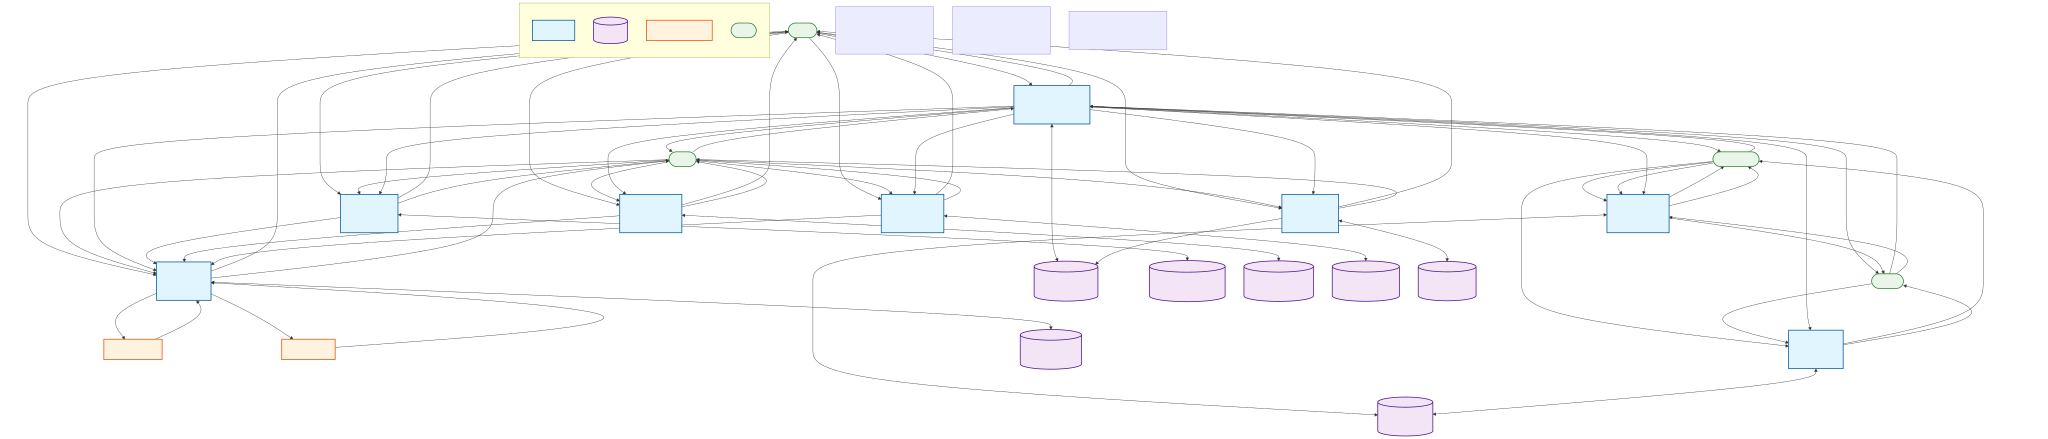
\includegraphics[width=0.9\textwidth]{diagrams/data_flow_diagram.png}
\caption{System Data Flow Diagram}
\label{fig:data-flow-diagram}
\end{figure}

\section{Requirement Specifications}

\subsection{Common functions}

\subsubsection{UC-01 – Register Donor Account}

\renewcommand{\arraystretch}{1.5}
\begin{longtable}{|p{4.5cm}|p{10.5cm}|}
\hline
\textbf{UC ID and Name:} & UC-01 – Register Donor Account \\
\hline
\textbf{Created By:} & DatNT \\
\hline
\textbf{Date Created:} & 28/6 \\
\hline
\textbf{Primary Actor:} & Guest \\
\hline
\textbf{Secondary Actors:} & System \\
\hline
\textbf{Description:} & A new user registers using email, password, and date of birth. The system creates a Level 1 account with the "Donor" role. To upgrade to Level 2 (eligible for blood donation registration), the user must visit a certified medical facility for in-person identity and eligibility verification. \\
\hline
\textbf{Trigger:} & The user clicks the 'Register' button. \\
\hline
\textbf{Preconditions:} &
\begin{itemize}
  \item The user is not logged in
  \item The email is not already in use
\end{itemize} \\
\hline
\textbf{Postconditions:} &
\begin{itemize}
  \item A Level 1 donor account is created
  \item The user can log in
  \item The account remains ineligible for donation event registration until verified (Level 2)
\end{itemize} \\
\hline
\textbf{Normal Flow:} &
\begin{enumerate}
  \item User opens the registration page
  \item Fills in the form
  \item Submits the form
  \item System validates input and creates the account
\end{enumerate} \\
\hline
\textbf{Alternative Flows:} & None defined \\
\hline
\textbf{Exceptions:} &
\begin{itemize}
  \item EX-1: If the email is already in use, the system shows an error message: \textit{"Email is already in use. Please use another email."}
  \item EX-2: If the user is under the required age, the system shows an ineligibility message: \textit{"You are not eligible to register as a blood donor."}
  \item EX-3: If a database or server error occurs, the system shows a retry message: \textit{"A system error occurred. Please try again later."}
\end{itemize} \\
\hline
\textbf{Business Rules:} &
\begin{itemize}
  \item BR-21: Only Level 2 (verified) users can register for donation events
  \item BR-22: User profile must be accurate and match official documents (relevant for Level 2 verification)
\end{itemize} \\
\hline
\textbf{Assumptions:} &
\begin{itemize}
  \item The user provides a valid email and basic profile information
  \item Level 2 access requires identity and health status confirmation at a medical center
\end{itemize} \\
\hline
\textbf{Priority:} & High \\
\hline
\textbf{Frequency of Use:} & Daily \\
\hline
\end{longtable}





\subsubsection{UC-02 – Log In}


\renewcommand{\arraystretch}{1.5}
\begin{longtable}{|p{4.5cm}|p{10.5cm}|}
\hline
\textbf{UC ID and Name:} & UC-02 – Log In \\
\hline
\textbf{Created By:} & KhoaDD \\
\hline
\textbf{Date Created:} & 28/6 \\
\hline
\textbf{Primary Actor:} & Guest, Donor \\
\hline
\textbf{Secondary Actors:} & System \\
\hline
\textbf{Description:} & The user logs into the system using their email and password. Upon successful login, the system redirects the user to their personal dashboard. Account access may be limited based on verification level (Level 1 or Level 2). \\
\hline
\textbf{Trigger:} & The user submits the login form. \\
\hline
\textbf{Preconditions:} &
\begin{itemize}
  \item A registered account exists
  \item The user is not currently logged in
\end{itemize} \\
\hline
\textbf{Postconditions:} &
\begin{itemize}
  \item The user is authenticated
  \item The user is redirected to their personal dashboard
\end{itemize} \\
\hline
\textbf{Normal Flow:} &
\begin{enumerate}
  \item User opens the login form
  \item Enters email and password
  \item Submits the form
  \item The system validates the credentials and logs the user in
  \item User is redirected to the dashboard with access based on account verification level
\end{enumerate} \\
\hline
\textbf{Alternative Flows:} & None defined \\
\hline
\textbf{Exceptions:} &
\begin{itemize}
  \item EX-1: If the email or password is incorrect, show an error message: \textit{"Invalid email or password."}
  \item EX-2: If the system is unavailable (e.g., server error), show an error message: \textit{"Unable to connect. Please try again later."}
\end{itemize} \\
\hline
\textbf{Business Rules:} &
\begin{itemize}
  \item BR-24: Email must follow institutional format (e.g., *@gmail.com)
\end{itemize} \\
\hline
\textbf{Assumptions:} &
\begin{itemize}
  \item The account is active and verified
  \item The user provides correct credentials
\end{itemize} \\
\hline
\textbf{Priority:} & High \\
\hline
\textbf{Frequency of Use:} & Daily \\
\hline
\end{longtable}

\subsubsection{UC-03 – View Hospital Information}

\renewcommand{\arraystretch}{1.5}
\begin{longtable}{|p{4.5cm}|p{10.5cm}|}
\hline
\textbf{UC ID and Name:} & UC-03 – View Hospital Information \\
\hline
\textbf{Created By:} & AnPP \\
\hline
\textbf{Date Created:} & 28/6 \\
\hline
\textbf{Primary Actor:} & Guest \\
\hline
\textbf{Secondary Actors:} & None \\
\hline
\textbf{Description:} & The user views information about the hospital, including its services, location, and contact details. \\
\hline
\textbf{Trigger:} & The user accesses the homepage or selects the "About Us" section. \\
\hline
\textbf{Preconditions:} &
\begin{itemize}
  \item The system is online and accessible
\end{itemize} \\
\hline
\textbf{Postconditions:} &
\begin{itemize}
  \item Hospital information is displayed to the user
\end{itemize} \\
\hline
\textbf{Normal Flow:} &
\begin{enumerate}
  \item User opens the website
  \item Clicks on "About Us"
  \item The system displays hospital information
\end{enumerate} \\
\hline
\textbf{Alternative Flows:} & None defined \\
\hline
\textbf{Exceptions:} &
\begin{itemize}
  \item EX-1: If hospital data is unavailable, the system displays a default message or an error: \textit{"Hospital information is currently unavailable."}
\end{itemize} \\
\hline
\textbf{Business Rules:} &
\begin{itemize}
  \item BR-19: Only admins can make changes to system about hospital information
\end{itemize} \\
\hline
\textbf{Assumptions:} &
\begin{itemize}
  \item Hospital information is properly maintained and updated in the system
\end{itemize} \\
\hline
\textbf{Priority:} & Medium \\
\hline
\textbf{Frequency of Use:} & Occasional \\
\hline
\end{longtable}


\subsubsection{UC-04 – Read Blogs}

\renewcommand{\arraystretch}{1.5}
\begin{longtable}{|p{4.5cm}|p{10.5cm}|}
\hline
\textbf{UC ID and Name:} & UC-04 – Read Blogs \\
\hline
\textbf{Created By:} & AnPP \\
\hline
\textbf{Date Created:} & 29/6 \\
\hline
\textbf{Primary Actor:} & Guest \\
\hline
\textbf{Secondary Actors:} & System \\
\hline
\textbf{Description:} & The user reads educational blog posts related to blood donation. \\
\hline
\textbf{Trigger:} & The user clicks on the "Blog" section. \\
\hline
\textbf{Preconditions:} &
\begin{itemize}
  \item At least one blog post has been published
\end{itemize} \\
\hline
\textbf{Postconditions:} &
\begin{itemize}
  \item A list of blogs is displayed
  \item The user can read individual posts
\end{itemize} \\
\hline
\textbf{Normal Flow:} &
\begin{enumerate}
  \item User clicks "Blog"
  \item System displays list of available posts
  \item User selects and reads a blog
\end{enumerate} \\
\hline
\textbf{Alternative Flows:} &
\textbf{AF-1:} No blog posts available → Show message: \textit{"No blog content is currently available."} \\
\hline
\textbf{Exceptions:} &
\begin{itemize}
  \item EX-1: System error → Show message: \textit{"Unable to load blogs. Please try again later."}
\end{itemize} \\
\hline
\textbf{Business Rules:} &
\begin{itemize}
  \item BR-17: Only blog authors or admins can edit blog articles
\end{itemize} \\
\hline
\textbf{Assumptions:} &
\begin{itemize}
  \item Blog content is reviewed and approved before being published
\end{itemize} \\
\hline
\textbf{Priority:} & Medium \\
\hline
\textbf{Frequency of Use:} & Frequent \\
\hline
\end{longtable}


\subsubsection{UC-05 – Manage Personal Profile}

\renewcommand{\arraystretch}{1.5}
\begin{longtable}{|p{4.5cm}|p{10.5cm}|}
\hline
\textbf{UC ID and Name:} & UC-05 – Manage Personal Profile \\
\hline
\textbf{Created By:} & TuanTM \\
\hline
\textbf{Date Created:} & 28/6 \\
\hline
\textbf{Primary Actor:} & Donor \\
\hline
\textbf{Secondary Actors:} & System \\
\hline
\textbf{Description:} & The donor views and updates their personal profile, including contact information. \\
\hline
\textbf{Trigger:} & The user accesses the "My Profile" section. \\
\hline
\textbf{Preconditions:} &
\begin{itemize}
  \item The user is logged in to the system
\end{itemize} \\
\hline
\textbf{Postconditions:} &
\begin{itemize}
  \item Profile data is updated and saved successfully
\end{itemize} \\
\hline
\textbf{Normal Flow:} &
\begin{enumerate}
  \item User navigates to profile section
  \item Edits personal information
  \item Clicks "Save"
  \item System validates and saves changes
\end{enumerate} \\
\hline
\textbf{Alternative Flows:} &
\textbf{AF-1:} Invalid input (e.g., phone number format) → Show error: \textit{"Please correct the highlighted fields."} \\
\hline
\textbf{Exceptions:} &
\begin{itemize}
  \item EX-1: If update fails due to system error → Show error: \textit{"Failed to update profile. Please try again."}
\end{itemize} \\
\hline
\textbf{Business Rules:} &
\begin{itemize}
  \item BR-22: User profile information must be accurate and match official documents
\end{itemize} \\
\hline
\textbf{Assumptions:} &
\begin{itemize}
  \item Profile data is accurate and editable
\end{itemize} \\
\hline
\textbf{Priority:} & High \\
\hline
\textbf{Frequency of Use:} & Occasional \\
\hline
\end{longtable}


\section{Design Specifications}

\subsection{Authentication System}

\subsubsection{User Login}

This screen allows users to authenticate into the system with role-based access to appropriate functionalities.

\textbf{Related use cases:} UC-002 User Login

\paragraph{UI Design}

\begin{longtable}{|p{3cm}|p{3cm}|p{8cm}|}
\hline
\textbf{Field Name} & \textbf{Field Type} & \textbf{Description} \\
\hline
Username* & Text Box & User enters registered username or email address for authentication \\
\hline
Password* & Password Box & User enters password (masked input for security) \\
\hline
Login & Button & Submits authentication request to server \\
\hline
Register & Hyperlink & Redirects to user registration page for new users \\
\hline
Forgot Password? & Hyperlink & Initiates password reset process \\
\hline
\end{longtable}

\paragraph{Database Access}

\begin{longtable}{|p{3cm}|p{2cm}|p{9cm}|}
\hline
\textbf{Table} & \textbf{CRUD} & \textbf{Description} \\
\hline
Users & R & Verify username/email and password hash for authentication \\
\hline
Roles & R & Retrieve user role information for authorization \\
\hline
LoginActivity & C & Log login attempt for security audit \\
\hline
\end{longtable}

\paragraph{SQL Commands}

\begin{lstlisting}[language=SQL]
-- 1. Authenticate user credentials
SELECT u.UserID, u.Username, u.Email, u.IsActive, r.RoleName
FROM Users u 
INNER JOIN Roles r ON u.RoleID = r.RoleID
WHERE (u.Username = ? OR u.Email = ?) AND u.IsActive = 1

-- 2. Log login activity
INSERT INTO LoginActivity 
(UserID, UsernameAttempted, AttemptTime, IsSuccess, IPAddress, UserAgent)
VALUES (?, ?, GETDATE(), ?, ?, ?)
\end{lstlisting}

\subsection{Appointment Management}

\subsubsection{Appointment Booking}

This screen enables patients to book appointments with available doctors by selecting from available time slots.

\textbf{Related use cases:} UC-004 Book Appointment

\paragraph{UI Design}

\begin{longtable}{|p{3cm}|p{3cm}|p{8cm}|}
\hline
\textbf{Field Name} & \textbf{Field Type} & \textbf{Description} \\
\hline
Doctor Selection* & Dropdown & List of available doctors with specialties \\
\hline
Appointment Date* & Date Picker & Calendar widget for selecting appointment date \\
\hline
Available Time Slots* & Radio Buttons & Dynamic list of available time slots for selected doctor/date \\
\hline
Appointment Notes & Text Area & Optional notes about appointment purpose or concerns \\
\hline
Book Appointment & Button & Submit appointment booking request \\
\hline
Cancel & Button & Return to previous screen without booking \\
\hline
\end{longtable}

\paragraph{Database Access}

\begin{longtable}{|p{3cm}|p{2cm}|p{9cm}|}
\hline
\textbf{Table} & \textbf{CRUD} & \textbf{Description} \\
\hline
Users & R & Retrieve available doctors with their specialties \\
\hline
DoctorAvailabilitySlots & R,U & Query available slots and mark as booked \\
\hline
Appointments & C & Create new appointment record \\
\hline
Notifications & C & Schedule appointment reminder notifications \\
\hline
\end{longtable}

\paragraph{SQL Commands}

\begin{lstlisting}[language=SQL]
-- 1. Get available doctors
SELECT u.UserID, u.FirstName, u.LastName, dp.Bio, s.SpecialtyName
FROM Users u
INNER JOIN DoctorProfiles dp ON u.UserID = dp.UserID
LEFT JOIN Specialties s ON dp.SpecialtyID = s.SpecialtyID
WHERE u.RoleID = (SELECT RoleID FROM Roles WHERE RoleName = 'Doctor')
AND u.IsActive = 1

-- 2. Get available time slots
SELECT AvailabilitySlotID, SlotDate, StartTime, EndTime
FROM DoctorAvailabilitySlots
WHERE DoctorUserID = ? AND SlotDate = ? AND IsBooked = 0
ORDER BY StartTime

-- 3. Create appointment
INSERT INTO Appointments 
(PatientUserID, DoctorUserID, AvailabilitySlotID, AppointmentDateTime, 
 Status, AppointmentNotes, CreatedAt, UpdatedAt)
VALUES (?, ?, ?, ?, 'Scheduled', ?, GETDATE(), GETDATE())

-- 4. Update availability slot
UPDATE DoctorAvailabilitySlots 
SET IsBooked = 1, UpdatedAt = GETDATE()
WHERE AvailabilitySlotID = ?
\end{lstlisting}

\subsection{Patient Care System}

\subsubsection{Patient Records Management}

This screen provides comprehensive medical record management for HIV patients including treatment history and current medications.

\textbf{Related use cases:} UC-007 Manage Patient Records

\paragraph{UI Design}

\begin{longtable}{|p{3cm}|p{3cm}|p{8cm}|}
\hline
\textbf{Field Name} & \textbf{Field Type} & \textbf{Description} \\
\hline
Medical History & Text Area & Comprehensive medical history including HIV diagnosis details \\
\hline
Current Allergies & Text Area & Known allergies and adverse reactions \\
\hline
Current Medications & Text Area & List of current medications including ARV regimens \\
\hline
Blood Type & Dropdown & ABO blood type classification \\
\hline
Emergency Contact & Text Box & Emergency contact person name \\
\hline
Emergency Phone & Text Box & Emergency contact phone number \\
\hline
Clinical Notes & Text Area & Doctor's clinical observations and notes \\
\hline
Save Record & Button & Save medical record updates \\
\hline
View ARV Treatments & Button & Access HIV treatment management screen \\
\hline
\end{longtable}

\paragraph{Database Access}

\begin{longtable}{|p{3cm}|p{2cm}|p{9cm}|}
\hline
\textbf{Table} & \textbf{CRUD} & \textbf{Description} \\
\hline
PatientRecords & R,U & Retrieve and update patient medical records \\
\hline
ARVTreatments & R & Access HIV treatment history \\
\hline
MedicationRoutines & R & View current medication schedules \\
\hline
Users & R & Verify doctor access permissions \\
\hline
\end{longtable}

\paragraph{SQL Commands}

\begin{lstlisting}[language=SQL]
-- 1. Retrieve patient record
SELECT RecordID, PatientUserID, MedicalHistory, Allergies, 
       CurrentMedications, BloodType, EmergencyContact, 
       EmergencyPhone, Notes, UpdatedAt
FROM PatientRecords
WHERE PatientUserID = ?

-- 2. Update patient record
UPDATE PatientRecords
SET MedicalHistory = ?, Allergies = ?, CurrentMedications = ?,
    BloodType = ?, EmergencyContact = ?, EmergencyPhone = ?,
    Notes = ?, UpdatedAt = GETDATE()
WHERE PatientUserID = ?

-- 3. Get ARV treatment history
SELECT ARVTreatmentID, Regimen, StartDate, EndDate, 
       Adherence, SideEffects, IsActive
FROM ARVTreatments
WHERE PatientUserID = ?
ORDER BY StartDate DESC
\end{lstlisting}

\section{Appendix}

\subsection{Assumptions \& Dependencies}

\begin{itemize}
    \item \textbf{AS-1:} Microsoft SQL Server database is available and properly configured for healthcare data storage
    \item \textbf{AS-2:} SMTP email service is configured for sending appointment and medication reminders
    \item \textbf{AS-3:} System users have basic computer literacy and internet access
    \item \textbf{AS-4:} Clinic staff will receive training on HIV patient management workflows
    \item \textbf{DE-1:} Integration with existing hospital information systems may be required
    \item \textbf{DE-2:} HIPAA compliance requirements must be met for patient data protection
    \item \textbf{DE-3:} System depends on reliable internet connectivity for real-time operations
\end{itemize}

\subsection{Limitations \& Exclusions}

\begin{itemize}
    \item System does not include billing or insurance processing capabilities
    \item Laboratory result integration is not included in current scope
    \item Telemedicine or video consultation features are excluded
    \item Mobile application development is not part of initial release
    \item Integration with pharmacy systems for prescription management is excluded
    \item Advanced analytics and reporting dashboards are limited in scope
\end{itemize}

\subsection{Business Rules}

\begin{longtable}{|p{2cm}|p{3cm}|p{9cm}|}
\hline
\textbf{ID} & \textbf{Category} & \textbf{Rule Definition} \\
\hline
BR-016 & Data Security & All patient data must be encrypted at rest and in transit using AES-256 encryption \\
\hline
BR-017 & Access Control & Role-based access ensures patients can only view their own records unless explicitly shared \\
\hline
BR-018 & Appointment Scheduling & No overlapping appointments allowed for any doctor or patient \\
\hline
BR-019 & Medication Adherence & ARV medication reminders are mandatory for all HIV patients unless opted out \\
\hline
BR-020 & Record Retention & Patient medical records must be retained for minimum 7 years per healthcare regulations \\
\hline
BR-021 & Emergency Access & Emergency override allows authorized medical staff to access any patient record \\
\hline
BR-022 & Notification Preferences & Patients must be able to opt-out of non-critical notifications \\
\hline
BR-023 & Data Backup & Daily automated backups of all patient data with 30-day retention \\
\hline
\end{longtable}

\subsection{Technical Specifications}

\begin{itemize}
    \item \textbf{Backend Technology:} Spring Boot 3.x with Java 17
    \item \textbf{Frontend Technology:} React 18 with modern JavaScript (ES6+)
    \item \textbf{Database:} Microsoft SQL Server with T-SQL stored procedures
    \item \textbf{Authentication:} JWT (JSON Web Tokens) with BCrypt password hashing
    \item \textbf{API Architecture:} RESTful APIs with JSON data exchange
    \item \textbf{Security:} HTTPS/TLS encryption, CORS configuration, input validation
    \item \textbf{Deployment:} Containerized deployment ready (Docker compatible)
\end{itemize}

\end{document}